\chapter{Power Series, Taylor Series, and Maclaurin Series}

\section{Representing Complex Functions as Polynomials}
FIXME is this the best example I can think of? there's room for improvement here

Consider the function $f(x) = \frac{80}{1-x^2}$. Suppose this represents the 
rate at which a tub is filling (that is, $V'(t) = \frac{80}{1-t^2}$, where 
$V'$ is the rate of change of volume of water (in units of gallons per hour) 
in the tub for $0 \leq t < 1$ and $t$ is the time in hours). Suppose the tub 
starts off empty and you want to turn off the faucet when it is full. If this 
bathtub holds 80 gallons, when should you turn off the faucet? This may seem 
trivial, but it's more complicated than it seems! As you may have guessed, we 
need to set up an integral:
$$V(t) = \int_{0}^t \frac{80}{1-x^2}\,dx = 80$$
That is, we are looking for some $t$ such that the area under $V'(t)$ is equal 
to 80 gallons. Try to evaluate this integral without a calculator: it's 
difficult! It would be much easier to integrate a polynomial. This is where 
power series come in.

Power series allow us to approximate complex functions as polynomials. They 
take the general form $\sum_{n=0}^\infty a_n (x - c)^n$, where $c$ is some 
constant. We say the power series is "centered at $c$" (we will discuss this 
further in later sections). For now, we just want to demonstrate the usefulness 
of these series. 

The power series that approximates $V'(t) = \frac{80}{1-t^2}$ near $x = 0$ is 
$\sum_{n=0}^\infty 80x^n$ (see figure \ref{fig:taylorapprox}). Taking the 
$5^{th}$ order series (that is, $n = 5$), we can estimate the volume in the 
tub as:
$$V(t) \approx \int_{0}^t \left[80 + 80x + 80x^2 + 80x^3 + 80x^4 + 80x^5 
\right]\,dx = 80$$
While this \textit{looks} like a longer integral, it's actually much easier 
to evaluate! As you can determine for yourself, 
$$V(t) = 80t + 40t^2 + \frac{80}{3}t^3 + 20t^4 + 16t^5 + \frac{40}{3}t^6 = 80$$
And while it may be tedious to find a $t$ such that $V(t) = 80$ by hand, it is 
very easy for a computer! Using a calculator, we find that $V(t) = 80$ when $t 
= 0.63727$ hours (or  about 40 minutes)

\begin{figure}[htbp]
\centering
    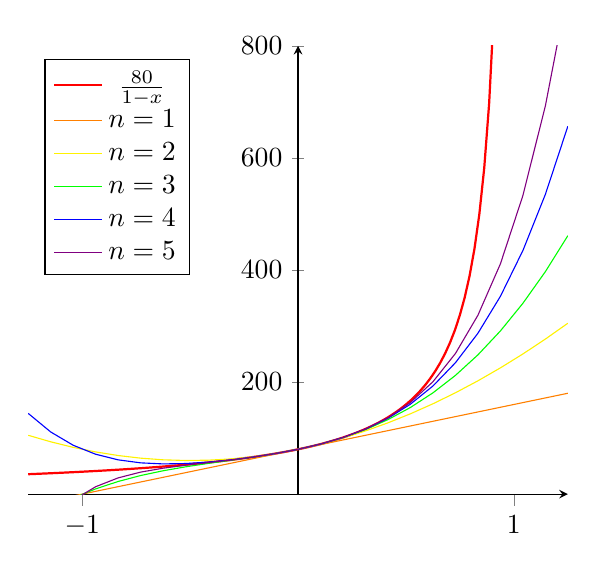
\begin{tikzpicture}
        \begin{axis}[axis lines = center, ymin = 0, ymax=800,
        xtick align = outside, xmin = -1.25, xmax = 1.25, 
        xtick = {-1, 1}, legend pos = north west]
        \addplot[red, thick, domain = -1.25:0.999, samples=100]{80/(1 - x)};
        \addlegendentry{$\frac{80}{1-x}$};
        \addplot[orange, domain = -1.25:1.25]{80+80*x};
        \addlegendentry{$n = 1$};
        \addplot[yellow, domain = -1.25:1.25]{80 + 80*x + 80*x^2};
        \addlegendentry{$n = 2$};
        \addplot[green, domain = -1.25:1.25]{80 + 80*x + 80*x^2 + 80*x^3};
        \addlegendentry{$n = 3$};
        \addplot[blue, domain = -1.25:1.25]{80 + 80*x + 80*x^2 + 80*x^3 + 80*x^4};
        \addlegendentry{$n = 4$};
        \addplot[violet, domain = -1.25:1.25]{80 + 80*x + 80*x^2 + 80*x^3 + 80*x^4 + 80*x^5};
        \addlegendentry{$n = 5$};
        \end{axis}
    \end{tikzpicture}
    \caption{$s_n = \sum_{i=0}^n 80x^i$ is a closer and closer approximation of 
    the function $f(x) = \frac{80}{1-x}$ near $x = 0$ as $n$ increases}
    \label{fig:taylorapprox}
\end{figure}

\section{Power Series}
Power series are series of the form \index{power series}
$$\sum_{n=0}^\infty c_n x^n = c_0 = c_1 x + c_2 x^2 + c_3 x^3 + \cdots + c_n 
x^n$$

for some fixed $x$. Depending on $x$, the series may converge or diverge. For 
example, the power series $\sum_{n=0}^\infty x^n$ converges for $ -1 < x < 1$ 
and diverges for all other values of $x$. This is because $\sum_{n=0}^\infty 
x^n$ is essentially a geometric series with $r = x$, which we already know 
converges for $|r|<1$. 

The form given above is for a power series centered on $0$, but a power series 
can be centered on any value, $a$. In that case, it looks like this:
$$\sum_{n=0}^\infty c_n (x - a)^n = c_0 + c_1(x - a) + c_2(x - a)^2 + \cdots + 
c_n(x - a)^n$$

Which we say is a \textit{power series in }$(x - a)$, or a \textit{power 
series centered at }$a$, or a \textit{power series about }$a$. 

\section{Power Series Convergence}
Sometimes, you'll be asked to find the value(s) of $x$ 
for which a power series converges. To do this, choose a test to apply and 
then find $x$ such that the test is passed. 

\textbf{Example}: For what values of $x$ is the series $\sum_{n=0}^\infty n!x^n$ 
convergent?

\textbf{Solution}: We will apply the Ratio Test (since there is a factorial in 
the series) and find $x$ such that $\lim_{n \to \infty} \left| \frac{a_{n+1}}{
a_n} \right| < 1$. 
$$\lim_{n \to \infty} \left| \frac{a_{n + 1}}{a_n} \right| = \lim_{n \to 
\infty} \left| \frac{(n+1)!x^{n+1}}{n!x^n} \right|$$
$$= \lim_{n \to \infty} \frac{(n+1) n! x \cdot x^n}{n!x^n} = \lim_{n \to 
\infty} \frac{(n+1) \cdot x}{1}$$
Which converges to $0$ when $x=0$ and diverges for all other values of $x$. 
Therefore, $\sum_{n=0}^\infty n!x^n$ converges if $x=0$. 

\textbf{Example}: For what values of $x$ does the series $\sum_{n=1}^\infty 
\frac{(x-4)^n}{2n}$ converge?

\textbf{Solution}: We will use the Ratio Test again. We are looking for an $x$ 
such that:
$$\lim_{n \to \infty} \left| \frac{a_{n+1}}{a_n} \right| < 1$$
$$\lim_{n \to \infty} \left| \frac{\frac{(x-4)^{n+1}}{2(n+1)}}{\frac{(x-4)^n}{
2n}} \right| < 1$$
$$\lim_{n \to \infty} \left| \frac{(x-4)(x-4)^n}{2n + 2} \cdot \frac{2n}{(x-4)^
n} \right| < 1$$
$$\lim_{n \to \infty} \left| \frac{(x-4)(x-4)^n(2n)}{(x-4)^n(2n+2)} \right| < 
1$$
$$\lim_{n \to \infty} \left| \frac{(x-4)(2n)}{2n + 2} \right| < 1$$
$$\lim_{n \to \infty} \left| \frac{2(x-4)}{2 + \frac{2}{n}} \right| < 1$$
$$2 \cdot \lim_{n \to \infty} \left| \frac{x-4}{1+ \frac{1}{n}} \right| < 1$$
$$2 \cdot \left| x-4 \right| < 1$$
$$\left| x-4 \right| < \frac{1}{2}$$\\
Which is true when 
$$-\frac{1}{2} < x-4 < \frac{1}{2}$$
$$3.5 < x < 4.5$$

We aren't done yet, though! We know the series converges for $3.5 < x < 4.5$ 
and diverges for $x < 3.5$ and $x > 4.5$. What about when $x = 3.5$ and $x = 
4.5$? (These are the cases where the Ratio Test is indeterminate, because 
$\lim_{n \to \infty} \left| \frac{a_{n+1}}{a_n} \right| = 1$.) We need to test 
each case. Substituting $x = 3.5$ into the series yields:
$$\sum_{n=1}^\infty \frac{(3.5-4)^n}{2n} = \sum_{n=1}^\infty \frac{\left( 
\frac{-1}{2} \right)^n}{2n}$$
$$= \sum_{n=1}^\infty \frac{(-1)^n}{n \cdot 2^{n+1}}$$
This is an alternating series, so we apply the alternating series test. First, 
we check that $|a_{n+1}| < |a_n|$:
$$\frac{1}{(n+1) \cdot 2^{n+2}}  < \frac{1}{n \cdot 2^{n+1}}$$
Which is true for all $n > 0$. Now we check if $\lim_{n \to \infty} |a_n| = 0$:
$$\lim_{n \to \infty} \frac{1}{n \cdot 2^{n+1}} = \frac{1}{\infty} = 0$$
Therefore, $\sum_{n=1}^\infty \frac{(-1)^n}{n \cdot 2^{n+1}}$ is convergent 
and $\sum_{n=1}^\infty \frac{(x-4)^n}{2n}$ is convergent for $x = 3.5$. Now we 
test $x=4.5$ for convergence:
$$\sum_{n=1}^\infty \frac{(4.5-4)^n}{2n} = \sum_{n=1}^\infty \left( 
\frac{1}{2} \right)^n \cdot \frac{1}{2n} = \sum_{n=1}^\infty \left( 
\frac{1}{2} \right)^{n+1} \frac{1}{n}$$
This series is less than the harmonic series $\sum_{n=1}^\infty \frac{1}{n}$ 
for all $n$. We know the harmonic series diverges, therefore by the direct 
comparison test, $\sum_{n=1}^\infty \left( \frac{1}{2} \right)^{n+1} 
\frac{1}{n}$ must also diverge. So our final answer to the original question 
is that the series is convergent fort $3.5 \leq x < 4.5$. 

\subsection{Radius of Convergence}
There are three possible outcomes when testing a power series $\sum_{n=0}^
\infty c_n (x-a)^n$ for convergence:
\begin{enumerate}
\item The series only converges for $x = a$
\item The series converges for all $x$
\item The series converges if $|x - a| < R$ and diverges for $|x - a| > R$, 
where $R$ is some positive number
\end{enumerate}

We call $R$ the \textbf{radius of convergence} \index{radius of convergence}. 
If we rearrange $|x - a| < R$, we can see why this is called a radius (see 
figure \ref{fig:radiusofconv}): 
$$a - R < x < a + R$$

\begin{figure}[htbp]
\centering
    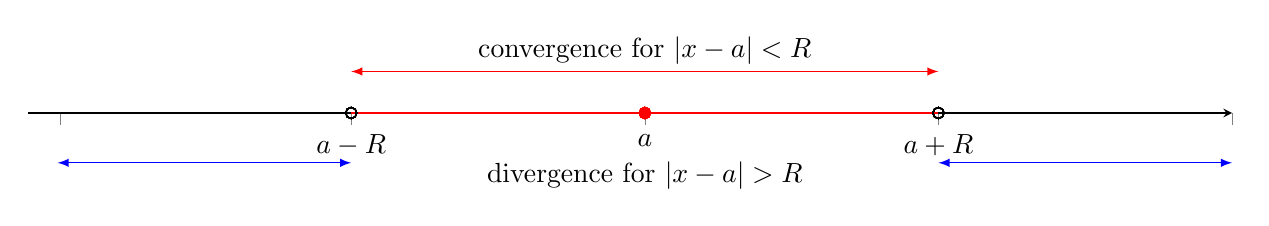
\begin{tikzpicture}
        \begin{axis}[axis y line = none, width = 2*\axisdefaultwidth, 
        height = 0.25*\axisdefaultwidth, axis lines = center, 
        xtick align = outside, xmin = -0.1, xmax = 4, 
        xtick = {0.01, 1, 2, 3, 4}, xticklabels = {, $a - R$, $a$, 
        $a + R$, }, ymin = -0.5, ymax = 0.5, 
        clip = false]
        \addplot[mark=o, black](1, 0);
        \addplot[mark=o, black](3, 0);
        \draw[red, thick] (1, 0) -- (3, 0);
        \addplot[mark=*, red] (2, 0);
        \node[] at (2, 1.5) {convergence for $|x - a| < R$};
        \draw[latex-latex, red] (1, 1) -- (3, 1);
        \node[] at (2, -1.5) {divergence for $|x - a| > R$};
        \draw[latex-latex, blue] (0, -1.2) -- (1, -1.2);
        \draw[latex-latex, blue] (3, -1.2) --(4, -1.2);
        \end{axis}
    \end{tikzpicture}
    \caption{$R$ is called the radius of convergence because it is half the 
    width of the window of convergence}
    \label{fig:radiusofconv}
\end{figure}

When $x = a \pm R$, the series could be convergent or divergent. You will need 
to test the endpoints of the windown of convergence to determine if the 
interval is open or closed. Thus, there are four possiblities for the interval 
of convergence:

\begin{enumerate}
\item $(a - R, a + R)$
\item$[a - R, a + R)$
\item$(a - R, a + R]$
\item$[a - R, a + r]$
\end{enumerate}

In the example of $\sum_{n=1}^\infty \frac{(x-4)^n}{2n}$ (shown above), 
$a = 4$ and $R = 0.5$ and we found that the power series is convergent for 
$x \in [3.5, 4.5)$. 

\textbf{Example}: For what values of $x$ is the Bessel function $J_0 (x) = 
\sum_{n=0}^\infty \frac{(-1)^n x^{2n}}{2^{2n}(n!)^2}$ convergent? 

\textbf{Solution}: Because there is a factorial, we will apply the Ratio Test:
$$\lim_{n \to \infty} \left| \frac{a_{n + 1}}{a_n} \right| <  1$$
$$\lim_{n \to \infty} \left| \frac{\frac{(-1)^{n + 1} x^{2(n + 1)}}{2^{2(n + 1
)}((n + 1)!)^2}}{frac{(-1)^n x^{2n}}{2^{2n}(n!)^2}} \right| < 1$$
$$\lim_{n \to \infty} \frac{x^{2n} x^2 2^{2n} n! n!}{2^{2n} 2^2 (n = 1)! (n + 
1)! x^{2n}} < 1$$
$$\lim_{n \to \infty} \frac{x^2 n! n!}{2^2 (n + 1)n! (n + 1)n!} < 1$$
$$\lim_{n \to \infty} \frac{x^2}{4(n + 1)^2} = 0 < 1$$
Because $lim_{n \to \infty} \left| \frac{a_{n + 1}}{a_n} \right| = 0$ for all 
$x$, the Bessel function $J_0 (x) = \sum_{n=0}^\infty \frac{(-1)^n x^{2n}}{2^{
2n}(n!)^2}$ is convergent for all real values of $x$ and the interval of 
convergence is $(-\infty, \infty)$. 

\textbf{Example}: Find the radius and interval of convergence for the series 
$\sum_{n=0}^\infty \frac{(-3)^n x^n}{\sqrt{n + 1}}$.

\textbf{Solution}: Again, we apply the ratio test to find values of $x$ such 
that $\lim_{n \to \infty} \left| \frac{a_{n + 1}}{a_n} \right| < 1$:
$$\lim_{n \to \infty} \left| \frac{(-3)^{n + 1} x^{n + 1}}{\sqrt{n + 1 + 1}} 
\cdot \frac{\sqrt{n + 1}}{(-3)^n x^n} \right| < 1$$
$$\lim_{n \to \infty} \left| \frac{(-3) x}{\sqrt{n + 2}} \cdot \frac{\sqrt{n + 
1}}{1} \right| < 1$$
$$\lim_{n \to \infty} \left| (-3)x \sqrt{\frac{n + 2}{n + 1}} \right| < 1$$
$$3|x| \lim_{n \to \infty} \sqrt{\frac{n + 2}{n + 1}} < 1$$
$$3|x| \lim_{n \to \infty} \sqrt{\frac{1 + 2/n}{1 + 1/n}} = 3|x|(1) < 1$$
$$3|x| < 1$$
$$|x| < \frac{1}{3}$$

Therefore, the radius of convergence is $\frac{1}{3}$. We need to test the 
endpoints, $x = \frac{-1}{3}$ and $x = \frac{1}{3}$ to determine the interval 
of convergence. First, we will test if $\sum_{n=0}^\infty \frac{(-3)^n x^n}{
\sqrt{n + 1}}$ when $x = \frac{-1}{3}$:
$$\sum_{n=0}^\infty \frac{(-3)^n \left( \frac{-1}{3} \right)^n}{\sqrt{n + 1}} 
= \sum_{n = 0}^\infty \frac{1^n}{\sqrt{n + 1}} = \sum_{n = 0}^\infty \frac{1}{
\sqrt{n + 1}}$$
This is a $p$-series such that $ p < 1$, so it is divergent and our original 
series does not converge for $x = \frac{-1}{3}$. Next we test $x = \frac{1}{3}$:
$$\sum_{n=0}^\infty \frac{(-3)^n \left( \frac{1}{3} \right)^n}{\sqrt{n + 1}} = 
\sum_{n = 0}^\infty \frac{(-1)^n}{\sqrt{n + 1}}$$
Which is an alternating series that converges by the alternating series test. 
Therefore, the interval of convergence for $\sum_{n=0}^\infty \frac{(-3)^n x^n}
{\sqrt{n + 1}}$ is $x \in \left( \frac{-1}{3}, \frac{1}{3} \right]$. 

\begin{Exercise}[label = radconv1]
[This problem was originally presented as a no-calculator, multiple-choice 
question on the 2012 AP Calculus BC exam.] What is the radius of convergence 
of the series $\sum_{n=0}^\infty \frac{(x - 4)^{2n}}{3^n}$?
\end{Exercise}

\begin{Answer}[ref = radconv1]
Since this sum has terms to the $n^{th}$ power, we will apply the Root Test, 
which states a series is convergent if $\lim_{n \to \infty} \sqrt[n]{\left| 
a_n \right|} < 1$. 
$$\lim_{n \to \infty} \sqrt[n]{\left| \frac{(x - 4)^{2n}}{3^n} \right|} < 1$$
$$\lim_{n \to \infty} \left| \frac{(x - 4) ^ {2n/n}}{3^{n/n}} \right| < 1$$
$$\lim_{n \to \infty} \frac{\left| (x-4)^2 \right|}{3} < 1$$
$$(x - 4)^2 < 3$$
$$\left| x - 4 \right| < \sqrt{3}$$
Therefore, the radius of convergence is $\sqrt{3}$. 
\end{Answer}

\begin{Exercise}[label = radconv2]
[This problem was originally presented as a no-calculator, multiple-choice 
question on the 2012 AP Calculus BC exam.] A power series is given by 
$\frac{x}{3} - \frac{x^3}{5} + \frac{x^5}{7} - \frac{x^7}{9} + \cdots$. Write 
the series in sigma notation and use the Ratio Test to determine the interval 
of convergence.
\end{Exercise}

\begin{Answer}[ref = radconv2]
We see that the series is alternating, so we know it involves $(-1)^n$ (we 
will begin indexing at $n = 0$). The powers of $x$ are given by $x^{2n+1}$ and 
the denominators are given by $2n + 3$. Therefore, the sum in sigma notation 
is $\sum_{n=0}^\infty (-1)^n \frac{x^{2n+1}}{2n+3}$. Applying the ratio test, 
the series is convergent when:
$$\lim_{n \to \infty} \left| \frac{(-1)^{n+1} x^{2(n+1)+1}}{2(n+1)+3} \frac{2n+
3}{(-1)^n x^{2n+1}} \right| < 1$$
$$\lim_{n \to \infty} \left| \frac{x^{2n+3}}{2n+5} \frac{2n+3}{x^{2n+1}} 
\right| < 1$$
$$\left| x^2 \right| \lim_{n \to \infty} \frac{2n+3}{2n+5} < 1$$
$$\left| x^2 \right| < 1$$
$$\left| x \right| < 1$$
So we know that the series is convergent on the open interval $x \in (-1, 1)$. 
We check the endpoints, $x = -1, 1$ for convergence. 
$$\sum_{n=0}^\infty \frac{(-1)^n (-1)^{2n+1}}{2n+3} = \sum_{n=0}^\infty \frac{
(-1)^{3n+1}}{2n+3}$$
When $x = -1$, the series is an alternating series such that $\left| a_{n+1} 
\right| < \left|a_n \right|$ and $\lim_{n \to \infty} a_n = 0$. Therefore, the 
series converges for $x = -1$.
$$\sum_{n=1}^\infty (-1)^n \frac{(1)^{2n+1}}{2n+3} = \sum_{n=1}^\infty \frac{
(-1)^n}{2n+3}$$
which is also an alternating series such that $\left| a_{n+1} \right| < \left| 
a_n \right|$ and $\lim_{n \to \infty} a_n = 0$. Therefore, the series 
converges for $x = 1$ and the interval of convergence is $x \in [-1, 1]$, 
which can also be written as $-1 \leq x \leq 1$. 
\end{Answer}

\section{Taylor and Maclaurin Series}

\begin{Exercise}[label = mac1]
[The problem was originally presented as a no-calculator, multiple-choice 
question on the 2012 AP Calculus BC exam.] The Maclaurin series for the 
function $f$ is given by $f(x) = \sum_{n=0}^\infty \left( -\frac{x}{4} \right)^
n$. What is the value of $f(3)$?
\end{Exercise}

\begin{Answer}[ref = mac1]
Substituting $x = 3$, the series is $\sum_{n=0}^\infty \left( -\frac{3}{4} 
\right)^n$, which is an alternating geometric series. Reindexing the series to 
begin at $n = 1$, this is equivalent to $\sum_{n = 1}^\infty \left( - 
\frac{3}{4} \right) ^ {n - 1}$, which is in the standard form $\sum_{n=1}^
\infty ar^{n-1}$ with $a = 1$ and $r = -\frac{3}{4}$. Then the value of the 
series is $\frac{a}{1-r} = \frac{1}{1-\left(- \frac{3}{4} \right)} = \frac{1}{1 
+ \frac{3}{4}} = \frac{1}{\frac{7}{4}} = \frac{4}{7}$. 
\end{Answer}

\begin{Exercise}[label = taylor1]
[This problem was originally presented as a calculator-allowed, multiple-choice 
question on the 2012 AP Calculus BC exam.] Let $f$ be function having 
derivatives of all orders for $x > 0$ such taht $f(3) = 2$, $f'(3) = -1$, 
$f''(3) = 6$, and $f'''(3) = 12$. Write a $3^{rd}$-degree Taylor polynomial 
for $f$ about $x = 3$ and estimate the value of $f(3.4)$
\end{Exercise}

\begin{Answer}[ref = taylor1]
A third-degree Taylor polynomial about $x = 3$ is given by $f(3) + \frac{
f'(3)}{1!} (x - 3) + \frac{f''(3)}{2!} (x - 3) ^ 2 + \frac{f'''(3)}{3!} (x - 3) 
^ 3$. Substituting what we know, they 3rd-degree Taylor polynomial is $f(x) 
\approx 2 + \frac{-1}{1} (x - 3) + \frac{6}{2} (x - 3) ^ 2 + \frac{12}{6}(x - 
3) ^ 3 = 2 - (x - 3) + 3 (x - 3) ^ 2 + 2 (x - 3) ^ 3$. Substituting $x = 3.5$, 
we find that $f(3.5) \approx 2 - (3.5 - 3) + 3 ( 3.5 - 3) ^ 2 + 2 (3.5 - 3) ^ 3 
= 2 - \frac{1}{2} + 3 \frac{1}{4} + 2\frac{1}{8} = 2 - \frac{1}{2} + 
\frac{3}{4} + \frac{1}{4} = 2.5$.
\end{Answer}

\begin{Exercise}[label = taylor2]
[This problem was originally presented as a calculator-allowed, free-response 
question on the 2012 AP Calculus BC exam.] The function $f$ is twice 
differentiable for $x > 0$ with $f(1) = 15$, $f'(1) = 8$, and $f''(1) = 20$. 
Write the second-degree Taylor polynomial about $x = 1$ and use it to 
estimate $f(1.4)$.
\end{Exercise}

\begin{Answer}
A second-degree Taylor polynomial about $x = 1$ is given by $f(x) \approx f(1) 
+ \frac{f'(1)}{1!}(x - 1) + \frac{f''(1)}{2!}(x - 1)^2 = 15 + 8(x - 1) + 10(x 
- 1)^2$. Substituting $x = 1.4$, we find that $f(1.4) \approx 15 + 8(1.4 - 1) 
+ 10(1.4 - 1)^2 = 19.8$.
\end{Answer}


